\documentclass[draft,linenumbers]{agujournal2018}
\usepackage{apacite}
\usepackage{url} %this package should fix any errors with URLs in refs.

%%%%%%%
% \usepackage{trackchanges}
% uncomment the line above to use the TrackChanges package to mark revisions if needed.
% The trackchanges package adds five new LaTeX commands:
%
%  \note[editor]{The note}
%  \annote[editor]{Text to annotate}{The note}
%  \add[editor]{Text to add}
%  \remove[editor]{Text to remove}
%  \change[editor]{Text to remove}{Text to add}
%
% complete documentation is here: http://trackchanges.sourceforge.net/
%%%%%%%

\draftfalse

\journalname{Space Weather}

\begin{document}
\title{A Test of the Frequency Independence Assumption of the System Parameters used in Geomagnetically Induced Current Calculations}

%% ------------------------------------------------------------------------ %%
%
%  AUTHORS AND AFFILIATIONS
%
%% ------------------------------------------------------------------------ %%

% Authors are individuals who have significantly contributed to the
% research and preparation of the article. Group authors are allowed, if
% each author in the group is separately identified in an appendix.)

% List authors by first name or initial followed by last name and
% separated by commas. Use \affil{} to number affiliations, and
% \thanks{} for author notes.
% Additional author notes should be indicated with \thanks{} (for
% example, for current addresses).

% Example: \authors{A. B. Author\affil{1}\thanks{Current address, Antartica}, B. C. Author\affil{2,3}, and D. E.
% Author\affil{3,4}\thanks{Also funded by Monsanto.}}

\authors{R.S. Weigel\affil{1} and P.J. Cilliers\affil{2}}

\affiliation{1}{Space Weather Lab, George Mason University}
\affiliation{2}{South African National Space Agency}

\affiliation{1}{4400 University Drive, Fairfax VA 22030}
\affiliation{2}{Hospital Street, Hermanus 7200}

%(repeat as many times as is necessary)

%% Corresponding Author:
% Corresponding author mailing address and e-mail address:

% (include name and email addresses of the corresponding author.  More
% than one corresponding author is allowed in this LaTeX file and for
% publication; but only one corresponding author is allowed in our
% editorial system.)

% Example: \correspondingauthor{First and Last Name}{email@address.edu}

\correspondingauthor{R.S. Weigel}{rweigel@gmu.edu}

%  List up to three key points (at least one is required)
%  Key Points summarize the main points and conclusions of the article
%  Each must be 100 characters or less with no special characters or punctuation

\begin{keypoints}
\item The system parameters derived from GIC and geoelectric field measurements are frequency dependent
\item A model with frequency dependence significantly outperforms a frequency independent model in predicting GIC
\item The best predictions are found when the model input is not the measured geoelectric field but rather the geoelectric field predicted by a transfer function model driven by the geomagnetic field
\end{keypoints}

\begin{abstract}
A common assumption used in estimating geomagnetically induced currents (GICs) in a power system given a direct measurement or indirect estimate (via a magnetotelluric transfer function) of the horizontal geoelectric field components $E_x$ and $E_y$ on Earth’s surface is that the system is resistive. That is, the approximation GIC(t) = $a_oE_x(t) + b_oE_y(t)$ (Model 1) is used, where $a_o$ and $b_o$ are frequency independent network parameters at frequencies associated with significant amplitudes of the geoelectric field.  We provide the first test of this assumption using GIC measurements made in a 187 kV transformer connected to a $\sim$100 km line in Memanbetsu, Japan and geoelectric field measurements made at the Memanbetsu Magnetic Observatory $\sim$10 kilometers away.  We compute frequency dependent network parameters  $A(\omega)$ and $B(\omega)$ in Model 2, $GIC(\omega) = A(\omega)E_x(\omega) + B(\omega)E_y(\omega)$, and find that they are not frequency independent and that this model provides a significantly better representation of measured GIC.
\end{abstract}

\section{Introduction}

Geomagnetically induced currents (GICs) are electric currents in man-made conducting systems due to electric fields induced near Earth’s surface.  These fields are a result of time variations in ionospheric currents on timescales on the order of hours or less and the movement of Earth’s surface relative to slow-varying current systems in Earth’s ionosphere that are near stationary relative to the Sun [REF].  Of particular interest are currents induced in electric power systems as they can lead to system degradation, disruption, and failure \citep{Albertson1993,NERC2012}.  Accurate estimation of GICs given direct measurements of the electric field (or estimates based on the geomagnetic field) is important for power system design [REF] retrospective analysis [REF] and for the mitigation of the impacts of space weather on power systems.

A common assumption made in estimates of GIC using either measured or estimated values of E is that the power system is resistive or quasi-DC so that the relationship $GIC(t) = a_oE_x(t) + b_oE_y(t)$ holds \citep{Albertson1981,Lehtinen1985}.  The coefficients $a_o$ and $b_o$ can then be calculated analytically using information about the connectivity of the power lines and values of the conductor and transformer resistances using DC circuit methods [e.g., Boteler, 2014a; Boteler and Pirjola, 2014b]. This assumption has been used or stated in many works in the past decade, for example, \citet{Pulkkinen2007,Wik2008,Pulkkinen2010,Ngwira2011,Viljanen2012,Overbye2012}.

In this work, we use a unique dataset in which measurements of the geoelectric field and geomagnetic field were made near a site where GICs were being measured in a power system.  We first estimate the system parameters $a_o$ and $b_o$ using conventional methods, which assume that they are frequency independent.  Then, we use a model in which the system parameters are frequency dependent, compute the frequency dependence, and compare this model with the traditional resistive model. 

\section{Data}

The 1-second-cadence GIC data used in this paper span cover a total of 36 days across the 10 intervals: 2006-04-02 -- 2006-04-10, 2006-07-25 -- 2006-07-29, 2006-08-05 -- 2006-08-08, 2006-08-19 -- 2006-08-21, 2006-11-07 -- 2006-11-12, 2006-11-28 -- 2006-11-29, 2006-12-01 -- 2006-12-01, 2006-12-14 -- 2006-12-15, 2007-11-18 -- 2007-11-20, and 2007-11-22 -- 2007-11-22 that have been presented previously in \citet{Watari2009} and \cite{Watari2015}.

One-second-cadence geoelectric field and geomagnetic field data were obtained from the Kakioka Magnetic Observatory of the Japan Meteorological Agency data portal. Data for the longest continuous time span, 2006-04-02 through 2006-04-10 are shown in the top and middle panels of Figure 1.

\begin{figure}[h]
\centering
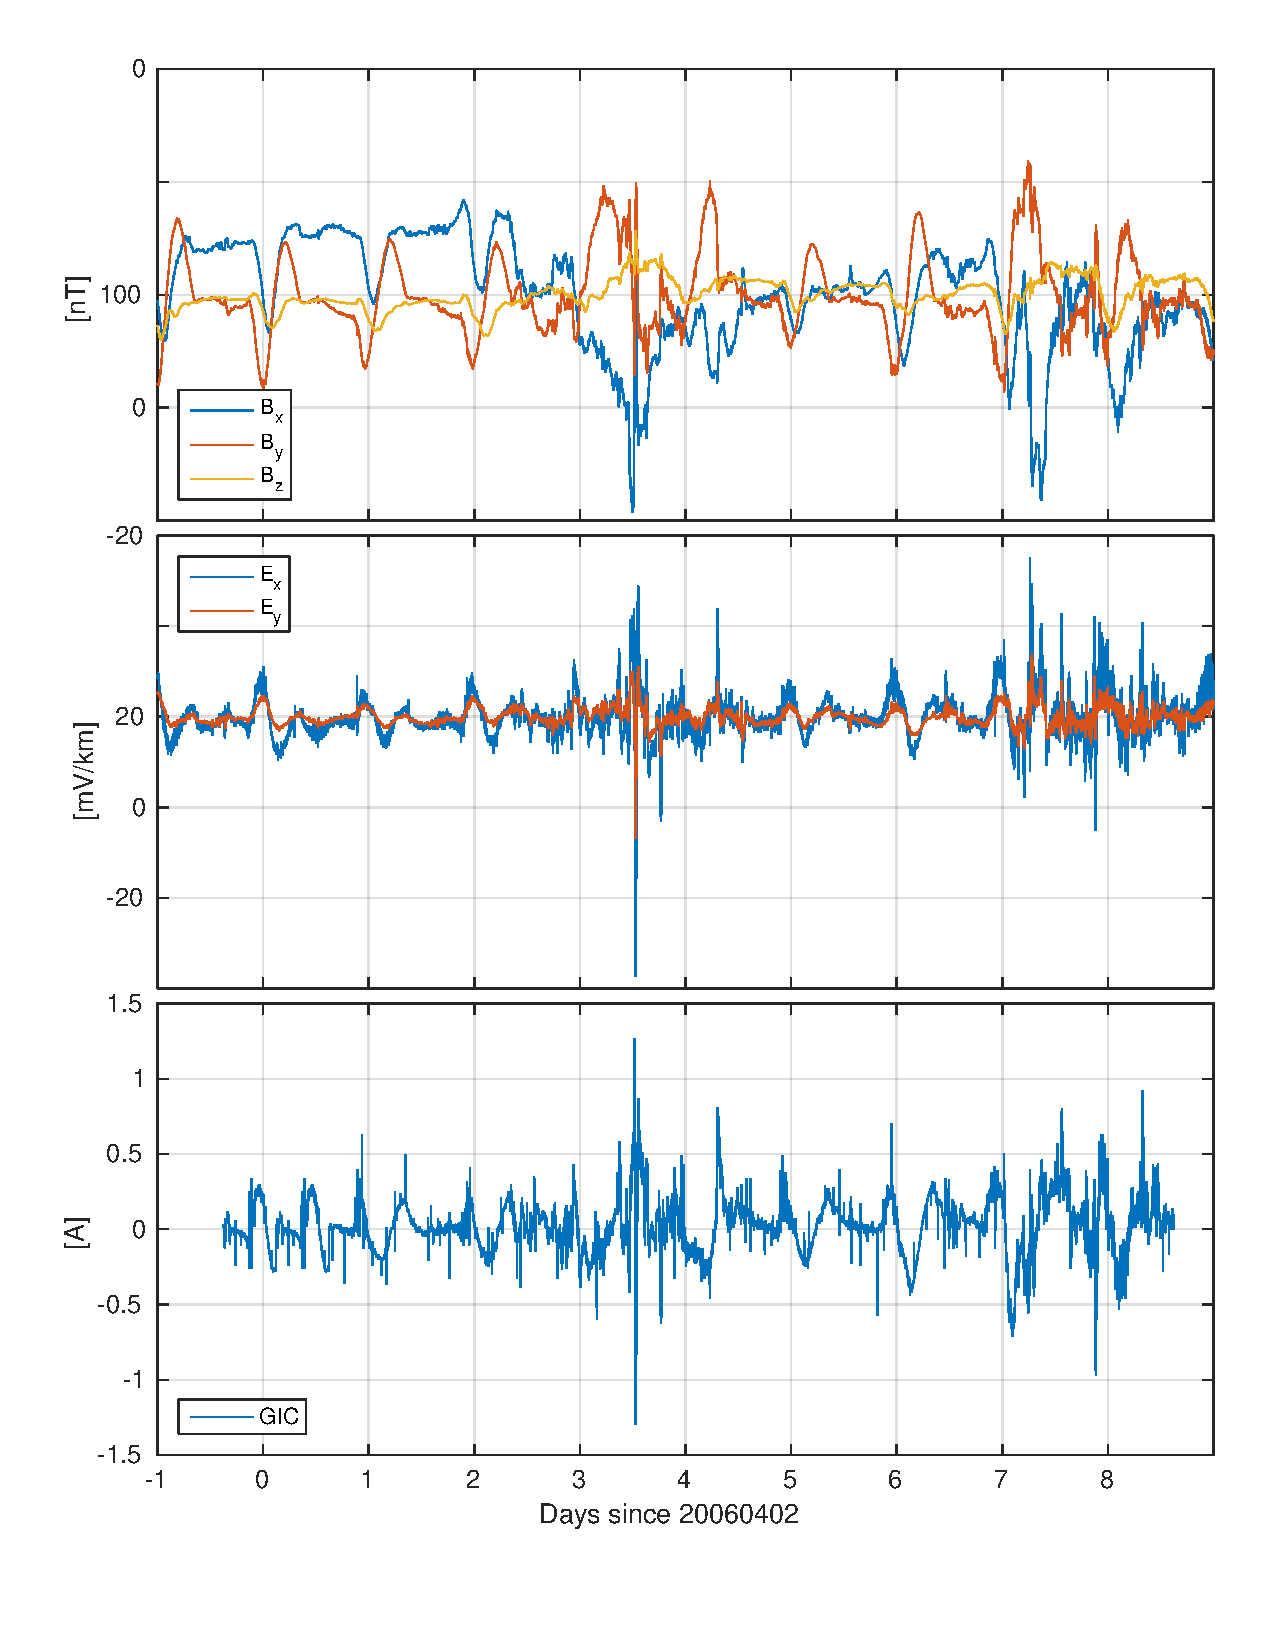
\includegraphics[]{figures/plot_raw_All_20060402.pdf}
\caption{(Top) One-second-cadence geomagnetic field measured at the Memanbetsu Magnetic Observatory (MMB). (Middle) One-second-cadence geoelectric field measured at the Memanbetsu Magnetic Observatory (MMB) X km from the Memanbetsu substation. (Bottom) One-second-cadence GIC measurements measured in a grounded neutral point of a Y-connected three-phase transformer connected to a 187 kV bus at the Memanbetsu substation of the Hokkaido Power Co.}
\label{figure1}
\end{figure}

The GIC dataset includes 1-second raw data and a 1 Hz low-pass filtered raw measurements.  The results presented here are for the 1 Hz low-pass filtered GIC values and data for the time interval 2006-04-02 through 2006-04-10 is shown in the bottom panel of Figure 1.

The GIC data contains non-physical spikes that are followed by a relaxation time of approximately 60 seconds. These spikes were removed by identifying times ts when the change in $|GIC|$ was greater than $0.04$ Amps and then data in a window $GIC(t_s-2)$ through $GIC(t_s+100)$ was replaced with a linear interpolation of the values from $GIC(t_s-3)$ to $GIC(t_s + 101)$.

Spikes in the electric field measurements were made using a similar procedure - when the absolute value of a component i of the electric field changed by more than 1 mV/km at time ts, the values $E_i(t_s-2)$ through $E_i(t_s+4)$ were replaced with a linear interpolation of the values from $E_i(t_s-3)$ to $E_i(t_s + 5)$.

The only modifications made to the magnetic field measurements was the replacement of 36 data points in all components of the magnetic field on 2006-08-06 with linearly interpolated values. The values for all components were the same and much larger than the surrounding values.

The subscripts $x$, $y$, and $z$ correspond to North, East, and Downward, respectively.

%Text here ===>>>

%%

%  Numbered lines in equations:
%  To add line numbers to lines in equations,
%  \begin{linenomath*}
%  \begin{equation}
%  \end{equation}
%  \end{linenomath*}



%% Enter Figures and Tables near as possible to where they are first mentioned:
%
% DO NOT USE \psfrag or \subfigure commands.
%
% Figure captions go below the figure.
% Table titles go above tables;  other caption information
%  should be placed in last line of the table, using
% \multicolumn2l{$^a$ This is a table note.}
%
%----------------
% EXAMPLE FIGURE
%
% \begin{figure}[h]
% \centering
% when using pdflatex, use pdf file:
% \includegraphics[width=20pc]{figsamp.pdf}
%
% when using dvips, use .eps file:
% \includegraphics[width=20pc]{figsamp.eps}
%
% \caption{Short caption}
% \label{figone}
%  \end{figure}
%
% ---------------
% EXAMPLE TABLE
%
% \begin{table}
% \caption{Time of the Transition Between Phase 1 and Phase 2$^{a}$}
% \centering
% \begin{tabular}{l c}
% \hline
%  Run  & Time (min)  \\
% \hline
%   $l1$  & 260   \\
%   $l2$  & 300   \\
%   $l3$  & 340   \\
%   $h1$  & 270   \\
%   $h2$  & 250   \\
%   $h3$  & 380   \\
%   $r1$  & 370   \\
%   $r2$  & 390   \\
% \hline
% \multicolumn{2}{l}{$^{a}$Footnote text here.}
% \end{tabular}
% \end{table}

%% SIDEWAYS FIGURE and TABLE
% AGU prefers the use of {sidewaystable} over {landscapetable} as it causes fewer problems.
%
% \begin{sidewaysfigure}
% \includegraphics[width=20pc]{figsamp}
% \caption{caption here}
% \label{newfig}
% \end{sidewaysfigure}
%
%  \begin{sidewaystable}
%  \caption{Caption here}
% \label{tab:signif_gap_clos}
%  \begin{tabular}{ccc}
% one&two&three\\
% four&five&six
%  \end{tabular}
%  \end{sidewaystable}

%% If using numbered lines, please surround equations with \begin{linenomath*}...\end{linenomath*}
%\begin{linenomath*}
%\begin{equation}
%y|{f} \sim g(m, \sigma),
%\end{equation}
%\end{linenomath*}

%%% End of body of article

%%%%%%%%%%%%%%%%%%%%%%%%%%%%%%%%
%% Optional Appendix goes here
%
% The \appendix command resets counters and redefines section heads
%
% After typing \appendix
%
%\section{Here Is Appendix Title}
% will show
% A: Here Is Appendix Title
%
%\appendix
%\section{Here is a sample appendix}

%%%%%%%%%%%%%%%%%%%%%%%%%%%%%%%%%%%%%%%%%%%%%%%%%%%%%%%%%%%%%%%%
%
% Optional Glossary, Notation or Acronym section goes here:
%
%%%%%%%%%%%%%%
% Glossary is only allowed in Reviews of Geophysics
%  \begin{glossary}
%  \term{Term}
%   Term Definition here
%  \term{Term}
%   Term Definition here
%  \term{Term}
%   Term Definition here
%  \end{glossary}

%
%%%%%%%%%%%%%%
% Acronyms
%   \begin{acronyms}
%   \acro{Acronym}
%   Definition here
%   \acro{EMOS}
%   Ensemble model output statistics
%   \acro{ECMWF}
%   Centre for Medium-Range Weather Forecasts
%   \end{acronyms}

%
%%%%%%%%%%%%%%
% Notation
%   \begin{notation}
%   \notation{$a+b$} Notation Definition here
%   \notation{$e=mc^2$}
%   Equation in German-born physicist Albert Einstein's theory of special
%  relativity that showed that the increased relativistic mass ($m$) of a
%  body comes from the energy of motion of the body—that is, its kinetic
%  energy ($E$)—divided by the speed of light squared ($c^2$).
%   \end{notation}




%%%%%%%%%%%%%%%%%%%%%%%%%%%%%%%%%%%%%%%%%%%%%%%%%%%%%%%%%%%%%%%%
%
%  ACKNOWLEDGMENTS
%
% The acknowledgments must list:
%
% >>>>	A statement that indicates to the reader where the data
% 	supporting the conclusions can be obtained (for example, in the
% 	references, tables, supporting information, and other databases).
%
% 	All funding sources related to this work from all authors
%
% 	Any real or perceived financial conflicts of interests for any
%	author
%
% 	Other affiliations for any author that may be perceived as
% 	having a conflict of interest with respect to the results of this
% 	paper.
%
%
% It is also the appropriate place to thank colleagues and other contributors.
% AGU does not normally allow dedications.


\acknowledgments
Magnetic and electric field data made at the Kakioka Magnetic Observatory was obtained from the Japan Meteorological Agency data portal http://www.kakioka-jma.go.jp/obsdata/metadata/en.

%% ------------------------------------------------------------------------ %%
%% References and Citations

%%%%%%%%%%%%%%%%%%%%%%%%%%%%%%%%%%%%%%%%%%%%%%%
% BibTeX is preferred:
%
\bibliography{agusample.bib}
%
% no need to specify bibliographystyle
%%%%%%%%%%%%%%%%%%%%%%%%%%%%%%%%%%%%%%%%%%%%%%%



% Please use ONLY \citet and \citep for reference citations.
% DO NOT use other cite commands (e.g., \cite, \citeyear, \nocite, \citealp, etc.).
%% Example \citet and \citep:
%  ...as shown by \citet{Boug10}, \citet{Buiz07}, \citet{Fra10},
%  \citet{Ghel00}, and \citet{Leit74}.

%  ...as shown by \citep{Boug10}, \citep{Buiz07}, \citep{Fra10},
%  \citep{Ghel00, Leit74}.

\end{document}



More Information and Advice:

%% ------------------------------------------------------------------------ %%
%
%  SECTION HEADS
%
%% ------------------------------------------------------------------------ %%

% Capitalize the first letter of each word (except for
% prepositions, conjunctions, and articles that are
% three or fewer letters).

% AGU follows standard outline style; therefore, there cannot be a section 1 without
% a section 2, or a section 2.3.1 without a section 2.3.2.
% Please make sure your section numbers are balanced.
% ---------------
% Level 1 head
%
% Use the \section{} command to identify level 1 heads;
% type the appropriate head wording between the curly
% brackets, as shown below.
%
%An example:
%\section{Level 1 Head: Introduction}
%
% ---------------
% Level 2 head
%
% Use the \subsection{} command to identify level 2 heads.
%An example:
%\subsection{Level 2 Head}
%
% ---------------
% Level 3 head
%
% Use the \subsubsection{} command to identify level 3 heads
%An example:
%\subsubsection{Level 3 Head}
%
%---------------
% Level 4 head
%
% Use the \subsubsubsection{} command to identify level 3 heads
% An example:
%\subsubsubsection{Level 4 Head} An example.
%
%% ------------------------------------------------------------------------ %%
%
%  IN-TEXT LISTS
%
%% ------------------------------------------------------------------------ %%
%
% Do not use bulleted lists; enumerated lists are okay.
% \begin{enumerate}
% \item
% \item
% \item
% \end{enumerate}
%
%% ------------------------------------------------------------------------ %%
%
%  EQUATIONS
%
%% ------------------------------------------------------------------------ %%

% Single-line equations are centered.
% Equation arrays will appear left-aligned.

Math coded inside display math mode \[ ...\]
 will not be numbered, e.g.,:
 \[ x^2=y^2 + z^2\]

 Math coded inside \begin{equation} and \end{equation} will
 be automatically numbered, e.g.,:
 \begin{equation}
 x^2=y^2 + z^2
 \end{equation}


% To create multiline equations, use the
% \begin{eqnarray} and \end{eqnarray} environment
% as demonstrated below.
\begin{eqnarray}
  x_{1} & = & (x - x_{0}) \cos \Theta \nonumber \\
        && + (y - y_{0}) \sin \Theta  \nonumber \\
  y_{1} & = & -(x - x_{0}) \sin \Theta \nonumber \\
        && + (y - y_{0}) \cos \Theta.
\end{eqnarray}

%If you don't want an equation number, use the star form:
%\begin{eqnarray*}...\end{eqnarray*}

% Break each line at a sign of operation
% (+, -, etc.) if possible, with the sign of operation
% on the new line.

% Indent second and subsequent lines to align with
% the first character following the equal sign on the
% first line.

% Use an \hspace{} command to insert horizontal space
% into your equation if necessary. Place an appropriate
% unit of measure between the curly braces, e.g.
% \hspace{1in}; you may have to experiment to achieve
% the correct amount of space.


%% ------------------------------------------------------------------------ %%
%
%  EQUATION NUMBERING: COUNTER
%
%% ------------------------------------------------------------------------ %%

% You may change equation numbering by resetting
% the equation counter or by explicitly numbering
% an equation.

% To explicitly number an equation, type \eqnum{}
% (with the desired number between the brackets)
% after the \begin{equation} or \begin{eqnarray}
% command.  The \eqnum{} command will affect only
% the equation it appears with; LaTeX will number
% any equations appearing later in the manuscript
% according to the equation counter.
%

% If you have a multiline equation that needs only
% one equation number, use a \nonumber command in
% front of the double backslashes (\\) as shown in
% the multiline equation above.

% If you are using line numbers, remember to surround
% equations with \begin{linenomath*}...\end{linenomath*}

%  To add line numbers to lines in equations:
%  \begin{linenomath*}
%  \begin{equation}
%  \end{equation}
%  \end{linenomath*}



